\documentclass[25pt, a0paper, landscape]{tikzposter}
\tikzposterlatexaffectionproofoff
\usepackage[utf8]{inputenc}
\usepackage{authblk}
\makeatletter
\renewcommand\maketitle{\AB@maketitle} % revert \maketitle to its old definition
\renewcommand\AB@affilsepx{\quad\protect\Affilfont} % put affiliations into one line
\makeatother
\renewcommand\Affilfont{\Large} % set font for affiliations
\usepackage{amsmath, amsfonts, amssymb}
\usepackage{tikz}
\usepackage{pgfplots}
% align columns of tikzposter; needs two compilations
\usepackage[colalign]{column_aligned}

% tikzposter meta settings
\usetheme{Default}
\usetitlestyle{Default}
\useblockstyle{Default}


%%%%%%%%%%% redefine title matter to include one logo on each side of the title; adjust with \LogoSep
\makeatletter
\newcommand\insertlogoi[2][]{\def\@insertlogoi{\includegraphics[#1]{#2}}}
\newcommand\insertlogoii[2][]{\def\@insertlogoii{\includegraphics[#1]{#2}}}
\newlength\LogoSep
\setlength\LogoSep{-70pt}

\renewcommand\maketitle[1][]{  % #1 keys
    \normalsize
    \setkeys{title}{#1}
    % Title dummy to get title height
    \node[inner sep=\TP@titleinnersep, line width=\TP@titlelinewidth, anchor=north, minimum width=\TP@visibletextwidth-2\TP@titleinnersep]
    (TP@title) at ($(0, 0.5\textheight-\TP@titletotopverticalspace)$) {\parbox{\TP@titlewidth-2\TP@titleinnersep}{\TP@maketitle}};
    \draw let \p1 = ($(TP@title.north)-(TP@title.south)$) in node {
        \setlength{\TP@titleheight}{\y1}
        \setlength{\titleheight}{\y1}
        \global\TP@titleheight=\TP@titleheight
        \global\titleheight=\titleheight
    };

    % Compute title position
    \setlength{\titleposleft}{-0.5\titlewidth}
    \setlength{\titleposright}{\titleposleft+\titlewidth}
    \setlength{\titlepostop}{0.5\textheight-\TP@titletotopverticalspace}
    \setlength{\titleposbottom}{\titlepostop-\titleheight}

    % Title style (background)
    \TP@titlestyle

    % Title node
    \node[inner sep=\TP@titleinnersep, line width=\TP@titlelinewidth, anchor=north, minimum width=\TP@visibletextwidth-2\TP@titleinnersep]
    at (0,0.5\textheight-\TP@titletotopverticalspace)
    (title)
    {\parbox{\TP@titlewidth-2\TP@titleinnersep}{\TP@maketitle}};

    \node[inner sep=0pt,anchor=west] 
    at ([xshift=-\LogoSep]title.west)
    {\@insertlogoi};

    \node[inner sep=0pt,anchor=east] 
    at ([xshift=\LogoSep]title.east)
    {\@insertlogoii};

    % Settings for blocks
    \normalsize
    \setlength{\TP@blocktop}{\titleposbottom-\TP@titletoblockverticalspace}
}
\makeatother
%%%%%%%%%%%%%%%%%%%%%%%%%%%%%%%%%%%%%


% color handling
\definecolor{TumBlue}{cmyk}{1,0.43,0,0}
\colorlet{blocktitlebgcolor}{TumBlue}
\colorlet{backgroundcolor}{white}

\graphicspath{ {images/} }

% title matter
\title{Object Detection within a Robotic Application}

\author[1]{Chia-Wen Tsai}
\author[2]{Felizitas Kunz}
\author[1]{Christoph Caprano}
\author[1]{Oskar Haller}

\affil[1]{Technical University of Munich}
\affil[2]{Ludwig-Maximilians-University, Munich}

\insertlogoi[width=15cm]{tum_logo}
\insertlogoii[width=15cm]{tum_logo}

% main document
\begin{document}

\maketitle

\begin{columns}
    \column{0.5}
    \block{Introduction}{
    	Our idea was to teach a Braccio Robotic Arm to play the child's game pairs. It should detect the playing cards laying on the table, their position and the motif of a card and find the second one. The robot picks one playing card up, places it on the stack and searches for the second one within the remaining cards. For object detection YOLOv2-Real-Time-Object detection is used for transfer learning with datasets containing images of our playing cards. We trained our network with Google Cloud Service.
    }
    \block{Dataset}{
    	Datasets for the project could be divided into two parts. Darknet has pre-trained on the Pascal VOC 2007+2012, and we trained 30 images for each of the 10 classes of the playing cards.
    	\bfseries Add sample label from our dataset \normalfont
    	
%    	\begin{tikzfigure}[Images of 20 classes from Pasca VOC2012, which is : \\
%    	aeroplane, bicycle, bird, boat, bottle, bus, car, cat, chair, cow, diningtable, dog, horse, motorbike, person, pottedplant, sheep, sofa, train and tvmonitor. ]
%    		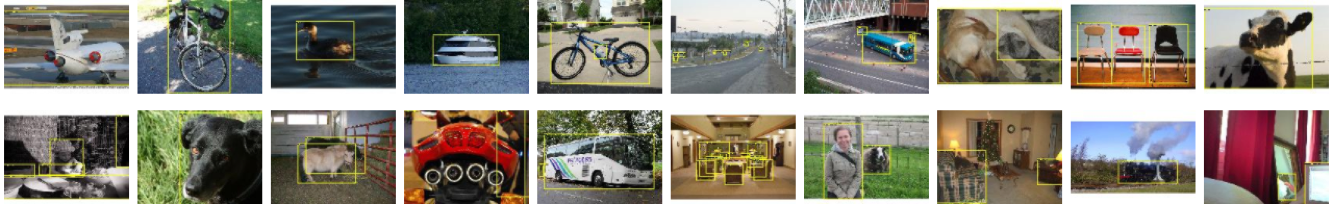
\includegraphics[width = 0.7\linewidth]{Pascal2012}
%    	\end{tikzfigure}

	    \begin{tikzfigure}[Training data of the playing cards. Ten classes of the cards are: \\
		Boat, Girl, Boy, Horse, EuropeanBird, PacificBird, Flower, BlueCard, Tree, Pineapple ]
	    	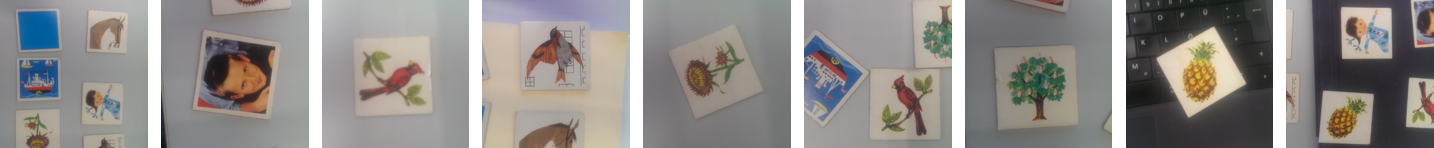
\includegraphics[width = 0.95\linewidth]{playingcard_data2}
	    \end{tikzfigure}
    }
    \block{Related Work}{
	  \begin{minipage}{\columnwidth}
	  		    	\begin{minipage}{800 pt}
	  		    		       	For the object detection, we used YOLOv2 respectivly Tiny YOLO with transfer learning to detect the motifs of the playing cards in real time.\\
	  		    		       	YOLOv2 trains the labels and the bounding boxes at the same time with a joint dataset consisting of one for classification and one for detection. If an image from the detection dataset is detected, it backpropagates normally. If the other case is detected, the network only backpropagates the classification specific parts.\\
	  		    		       A simplyfied network based on Goolenet architecture with additional features like batch normalization and high resolution classifiers makes YOLOv2 fast and accurate.
	  		    	\end{minipage}
	  		    	\hspace{50 pt}
	  		    	\begin{minipage}{500 pt}
	  		    		       	\begin{tikzfigure}[Network architecture. ]
	  		    		       		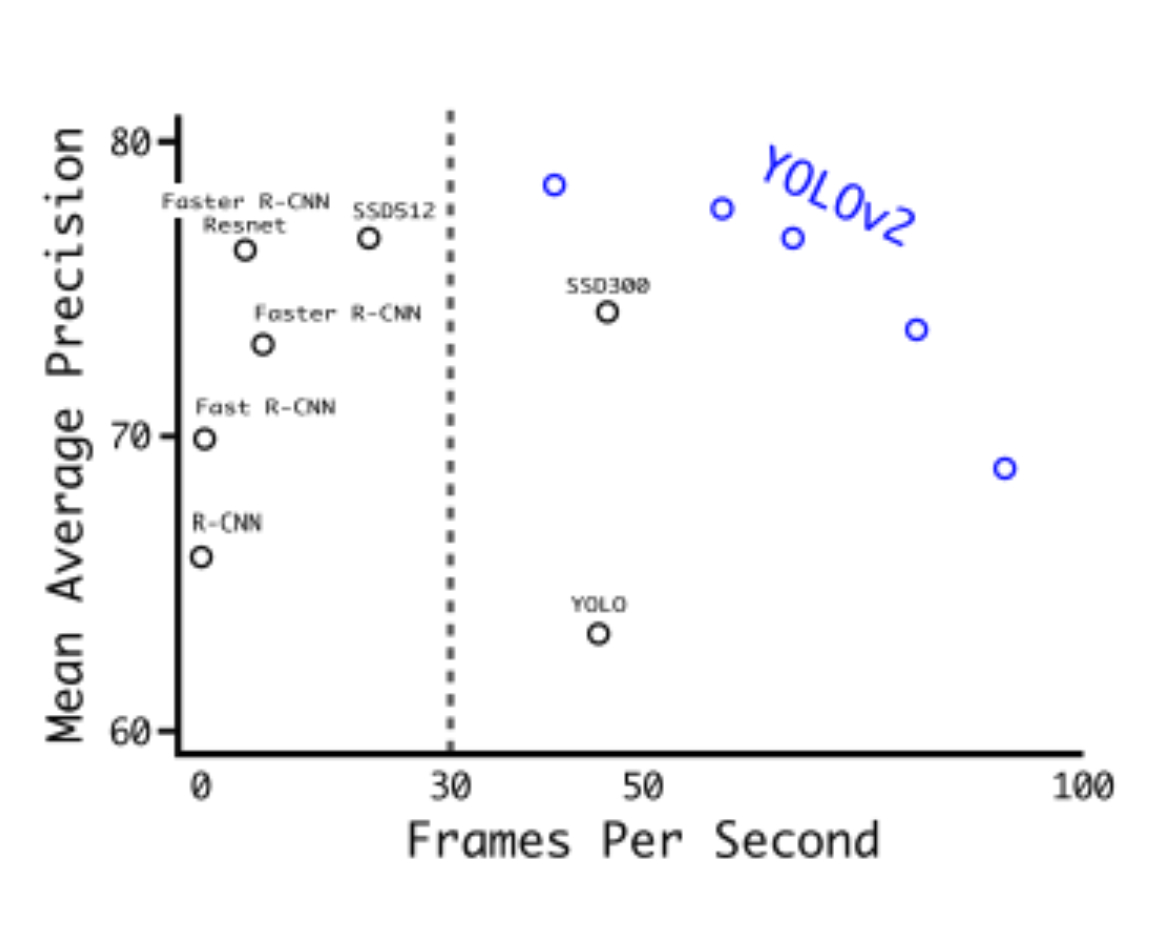
\includegraphics[width = 500 px]{images/YoloV2_Acc_Speed.jpg}
	  		    		       	\end{tikzfigure}
	  		    	\end{minipage}
	  \end{minipage}       	
    }

    \column{0.5}

    \block{Methodology}{
		     \bfseries{Network Architecture}\\
		     \normalfont
	    	\begin{tikzfigure}[Network architecture. ]
	    		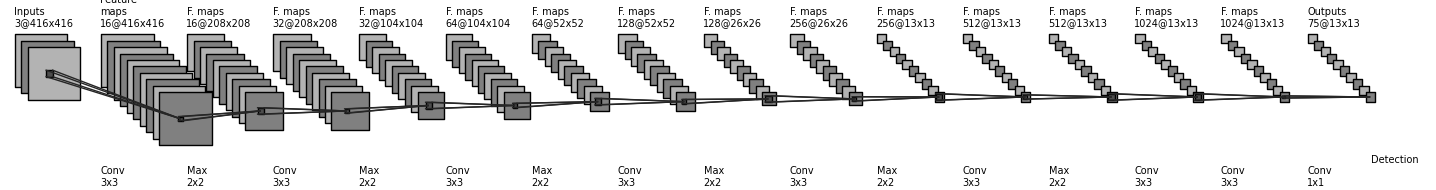
\includegraphics[width = \linewidth]{figure_tiny_yolo_webcam}
	    	\end{tikzfigure}
%   	    	\begin{tikzfigure}[System structure under ROS (Robot Operating System)]
%   	    		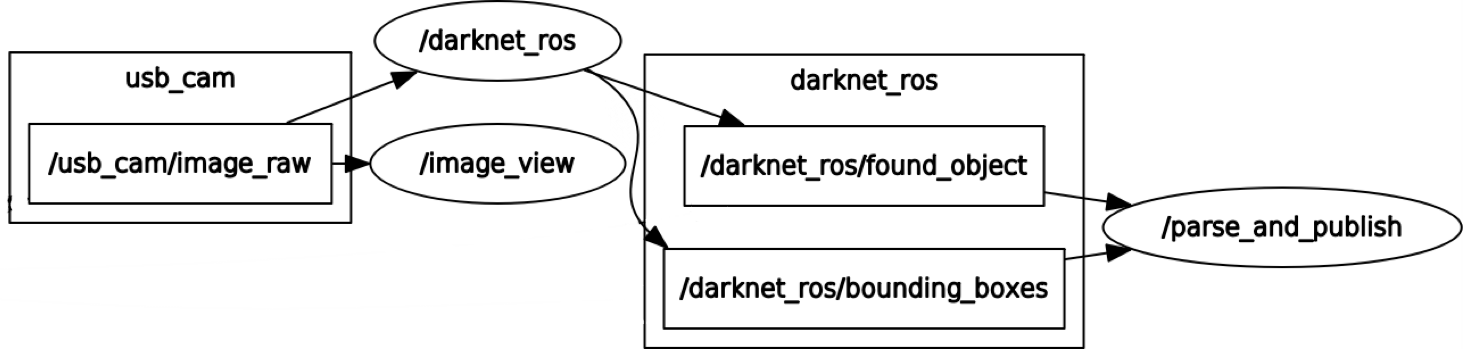
\includegraphics[width = 0.7\linewidth]{Rosgraph}
%   	    	\end{tikzfigure}
   	    	

 				\begin{minipage}{\columnwidth}
 					\begin{minipage}{800 pt}
			  	    	\begin{tikzfigure}[Hardware setup]
			  	    		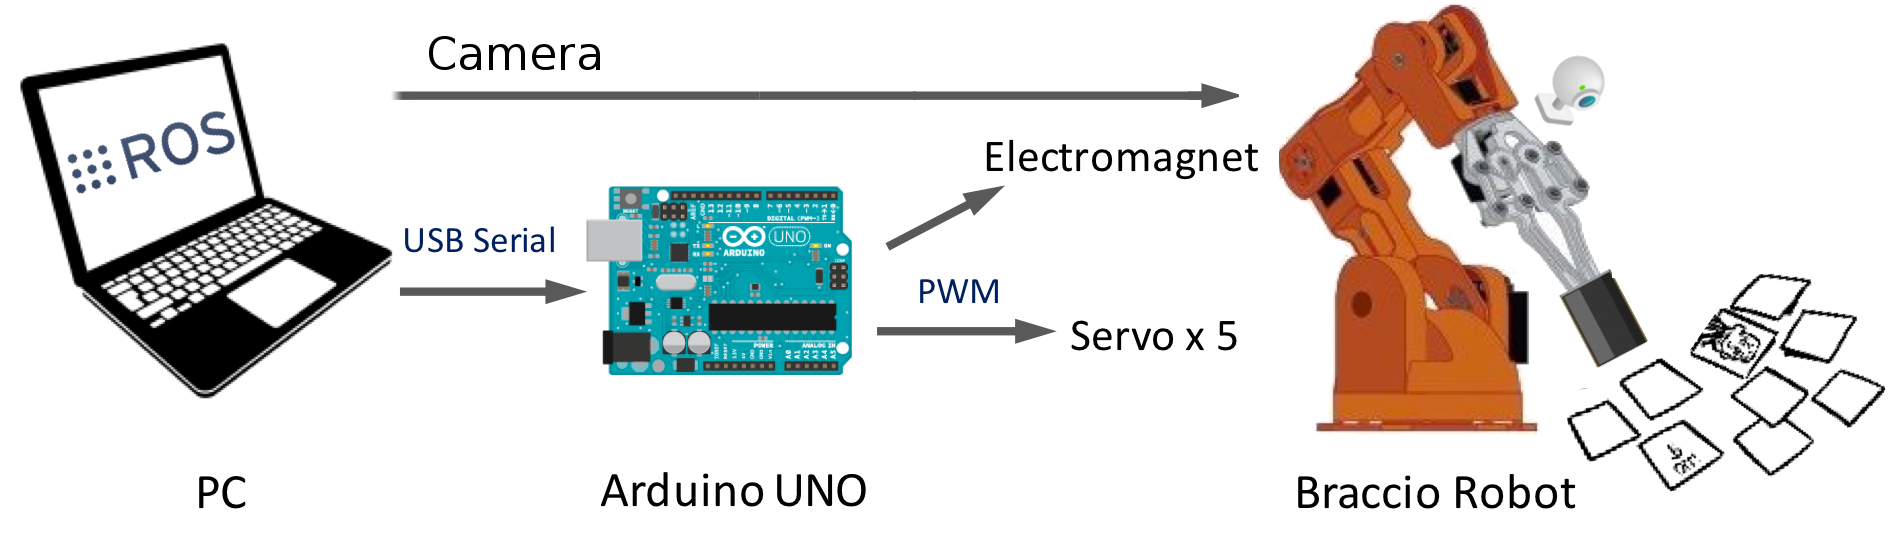
\includegraphics[width = 800 pt]{hardware_structure2}
			  	    	\end{tikzfigure}
 					\end{minipage}
 					\hspace{50 pt}
 					\begin{minipage}{500 pt}
 						\normalfont
						We used a pre-trained Tiny YOLO network (see figure 3). It has only 15 layers (Yolo has 30), which makes it much faster, but also less accurate. The architecture consits of 9 convolutional and 6 pooling layers. We adjusted some parameters \bfseries{which ones again? I forgot}\\
						\normalfont We trained the last two convolutional layers with our dataset to extract the middle and high level features. The results were very accurate.\\
						Our hardware architecture consists of a PC, an Arduino UNO, an electromagnet, a camera and the Braccio Robot Arm. They communicate with ROS.
 					\end{minipage}
 				\end{minipage}
    }
        \block{Outcome}{
			\begin{minipage}{\columnwidth}
			    		  	\begin{minipage}{800 pt}
				        	\begin{tikzfigure}
				        		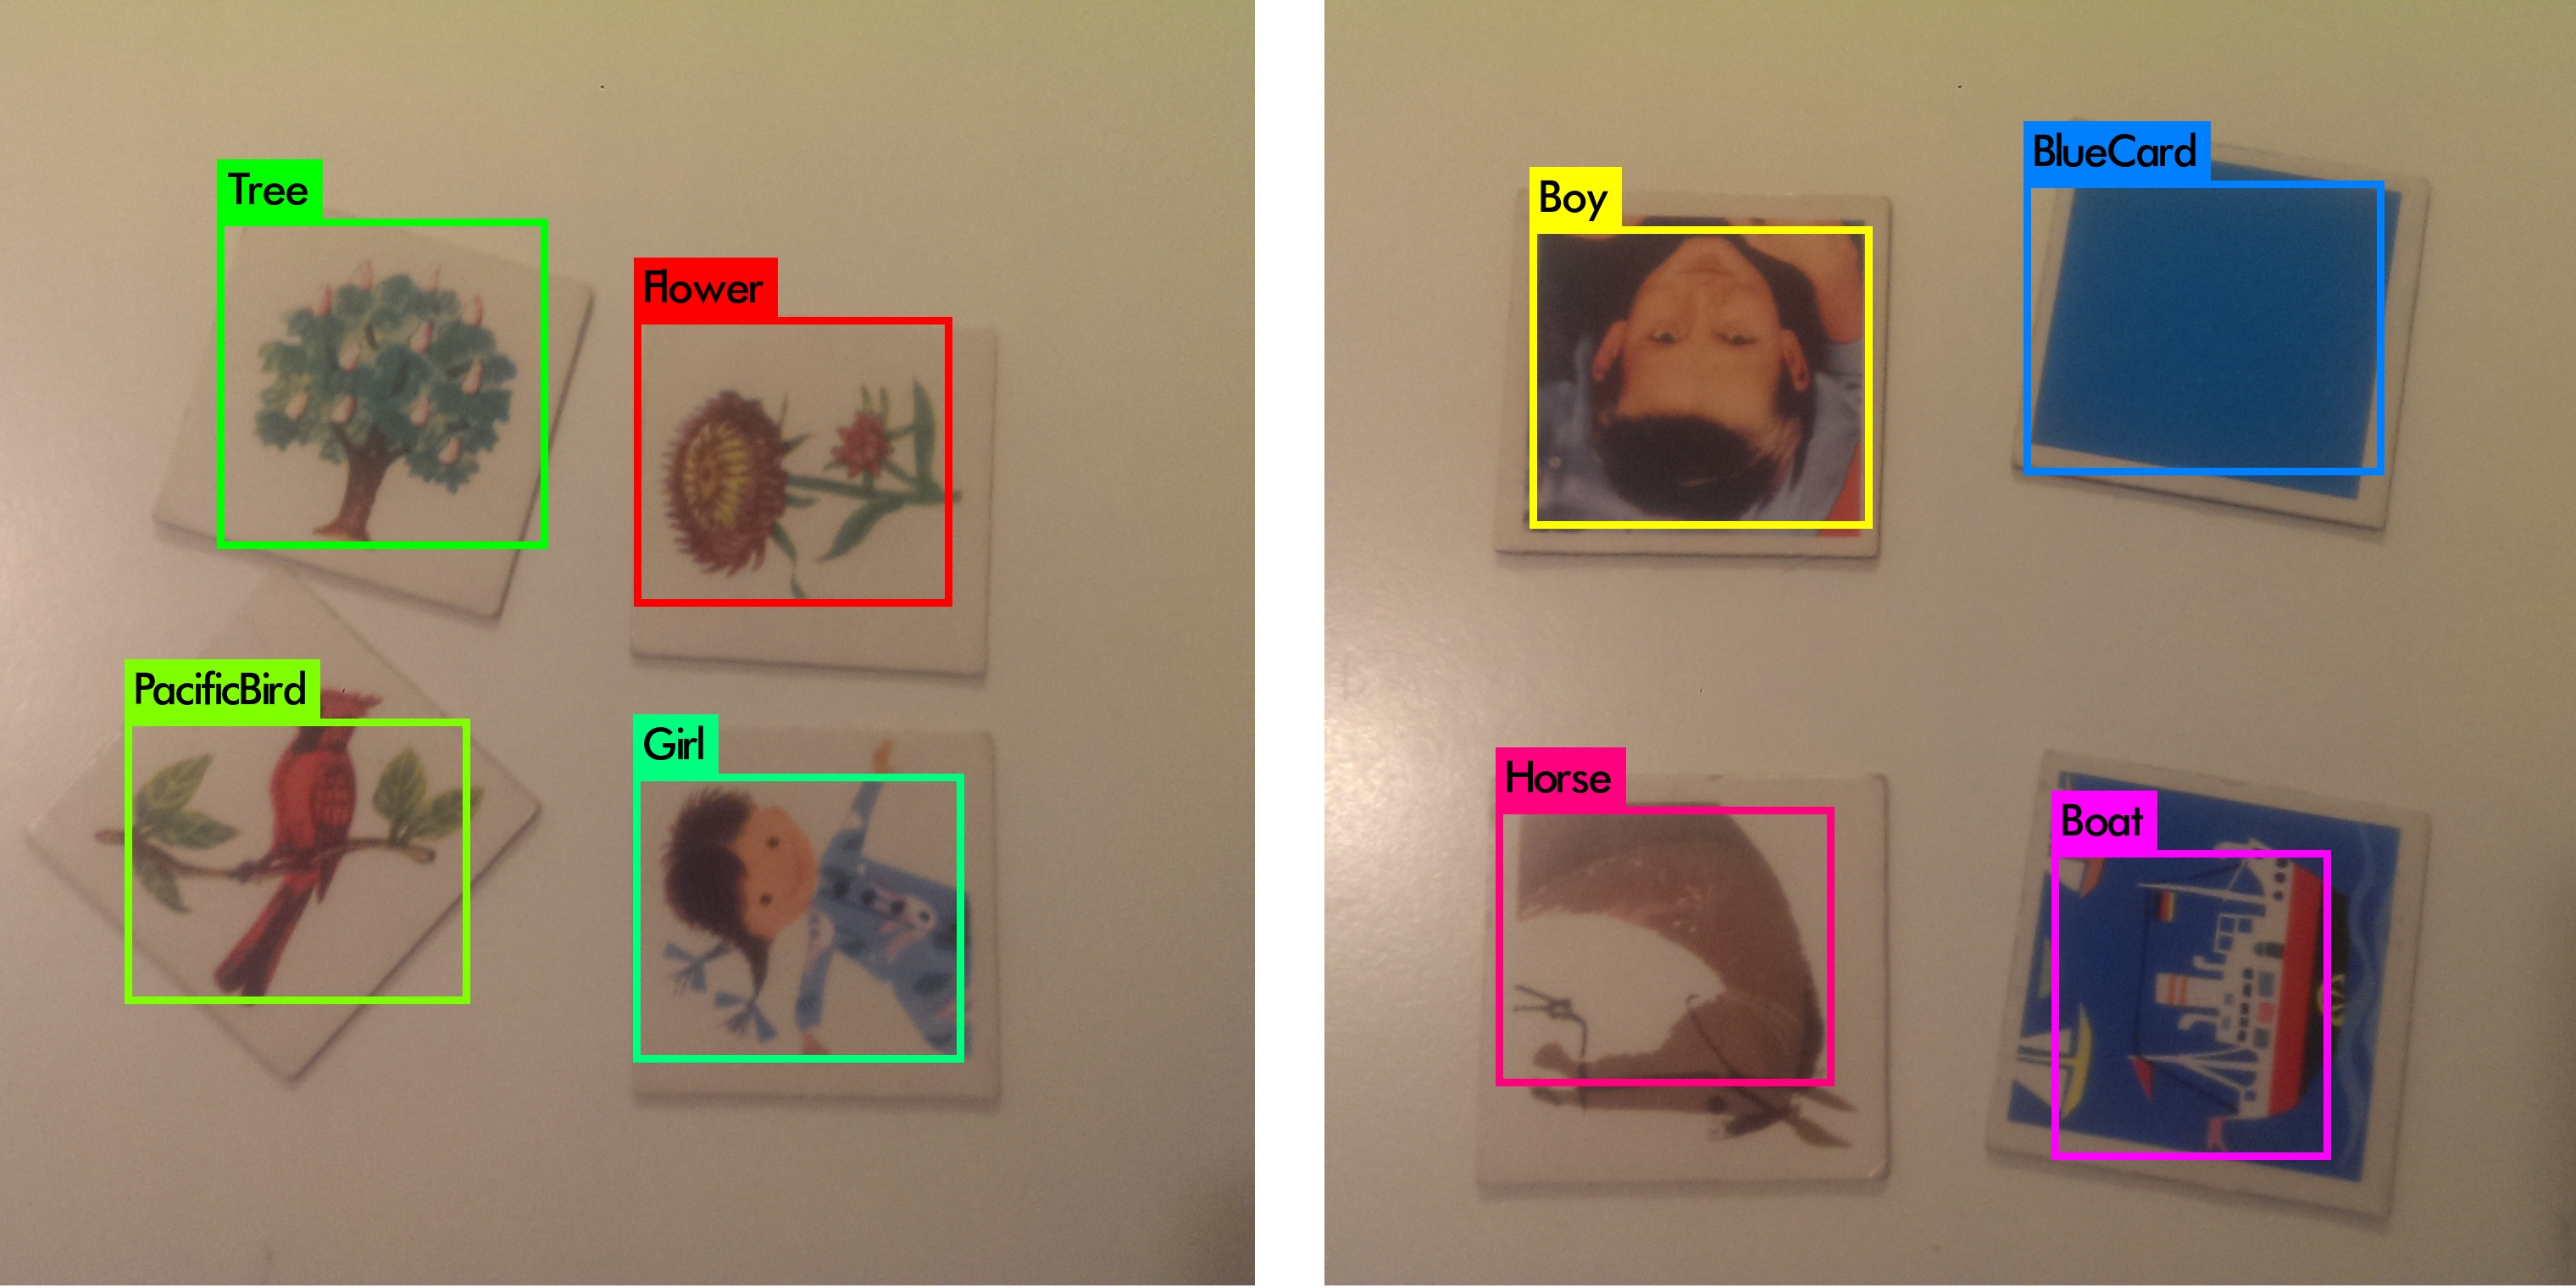
\includegraphics[height=300 px]{images/predictions3.jpg}
				        		\label{fig:predictions}
				        	\end{tikzfigure}
			    		  	\end{minipage}
			    		  	\hspace{50 pt}
			    		  	\begin{minipage}{500 pt}
					        	\begin{itemize}
					        		
					        		\item Network from Tiny YOLO
					        		
					        		\item 10 cards + classes
					        		
					        		\item Architecture
					        		
					        		
					        		\item Filters from results
					        		
					        		\item Camera input with detection labels
					        	\end{itemize}
			    		  	\end{minipage}
			\end{minipage}
			\bfseries Add image with weights
        }
\end{columns}

\end{document}
